\section{Modelagem}
Trataremos o problema descrito em sua forma discreta, i.e., dado um valor $\delta$ definimos uma malha quadriculada que cobre toda a regi\~{a}o de interesse como na Figura~\ref{fig:malha_quad}. Cada elemento da malha quadriculada recebe uma identificação numérica como ilustrada na Figura~\ref{fig:malha_quad_num}.
\begin{figure}[!htb]
    \centering
    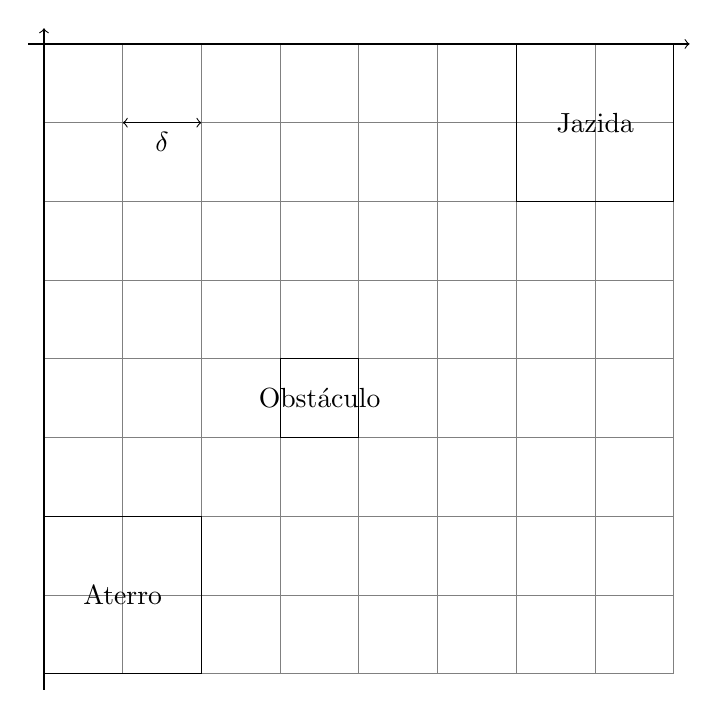
\begin{tikzpicture}
        \draw[color=gray] (0,0) grid (8,8);
        \draw[->] (-.2,8) -- (8.2,8);
        \draw[->] (0,-.2) -- (0,8.2);

        \draw (0,0) rectangle (2,2) node[midway]{Aterro};
        \draw (3,3) rectangle (4,4) node[midway]{Obst\'{a}culo};
        \draw (6,6) rectangle (8,8) node[midway]{Jazida};

        \draw[<->] (1,7) -- (2,7) node[midway, below]{$\delta$};
    \end{tikzpicture}
    \caption{Ilustra\c{c}\~{a}o da malha quadricular sobre a regi\~{a}o de interesse.}
    \label{fig:malha_quad}
\end{figure}
\begin{figure}[!htb]
    \centering
    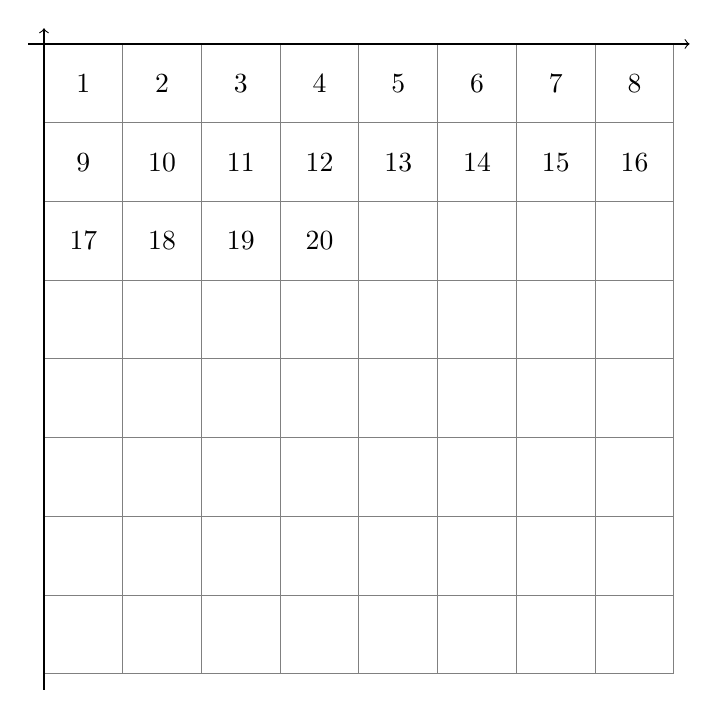
\begin{tikzpicture}
        \draw[color=gray] (0,0) grid (8,8);
        \draw[->] (-.2,8) -- (8.2,8);
        \draw[->] (0,-.2) -- (0,8.2);

        \foreach \x in {1,...,8}{
            \node at (\x - .5,7.5) {$\x$};
        }
        \foreach \x in {9,...,16}{
            \node at (\x - 8.5,6.5) {$\x$};
        }
        \foreach \x in {17,...,20}{
            \node at (\x - 16.5,5.5) {$\x$};
        }
    \end{tikzpicture}
    \caption{Ilustra\c{c}\~{a}o da numeração da malha quadricular.}
    \label{fig:malha_quad_num}
\end{figure}

% Tentar manter a mesma notação utilizada em ``A Linear Continuous Transportation Problem''
Seja $\phi, \psi: \mathbb{N} \to \mathbb{R}$ e $f: \mathbb{N}^2 \to \mathbb{R}$, onde $\phi(x)$ corresponde ao volume de solo disponível na célula $x$, $\psi(y)$ ao volume de solo necessário na célula $y$, $f(x,y)$ ao volume de solo transportado da célula $x$ para a célula $y$ e $d(x, y)$ a distância entre as células $x$ e $y$\footnote{A distância entre as células $x$ e $y$ será definida posteriormente.}. Seja também $D$ o comprimento dos canos disponíveis, $J$ o conjunto de células que compõem a jazida e $A$ o conjunto de células que compõem o aterro.

Então, podemos modelar o problema da seguinte forma
\begin{subequations}
    \begin{align}
        \text{min } & \sum_{x \in J} \sum_{y \in A} \xi_{x,y},
        \label{eq:model_without_obs:obj_func} \\
        \text{s.a. } & \xi_{x,y} \geq 0, && \forall x, y \in N,
        \label{eq:model_without_obs:var} \\
        & \xi_{x,y} = 0 && \forall d_{x,y} > D,
        \label{eq:model_without_obs:max_dist} \\
        & \sum_{y \in A} \xi_{x,y} \leq \phi(x), && \forall x \in J,
        \label{eq:model_without_obs:max_jazida} \\
        & \sum_{x \in J} \xi_{x,y} \leq \psi(y), && \forall y \in A,
        \label{eq:model_without_obs:max_aterro}
    \end{align}
    \label{eq:model_without_obs}
\end{subequations}

Ao utilizar a malha quadriculada podemos definir a dist\^{a}ncia entre dois quadrados da malha de pelo menos tr\^{e}s maneiras diferentes:
\begin{enumerate}
    \item $d_l$, que \'{e} a menor dist\^{a}ncia entre qualquer dois pontos dos quadrados,
    \item $d_u$, que \'{e} a maior dist\^{a}ncia entre qualquer dois pontos dos quadrados, e
    \item $d_c$, que \'{e} a dist\^{a}ncia entre os centros dos quadrados.
\end{enumerate}
Na Figura~\ref{fig:dist_malha} \'{e} ilustrado cada uma das dist\^{a}ncias acima descrita.
\begin{figure}[!htb]
    \centering
    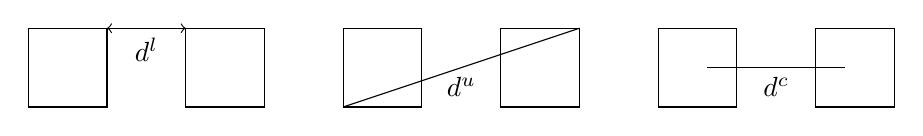
\begin{tikzpicture}
        \draw (0,0) rectangle (1,1);
        \draw (2,0) rectangle (3,1);
        \draw[<->] (1,1) -- (2,1) node[midway, below]{$d^l$};

        \draw (4,0) rectangle (5,1);
        \draw (6,0) rectangle (7,1);
        \draw (4,0) -- (7,1) node[midway, below]{$d^u$};

        \draw (8,0) rectangle (9,1) node[midway](A){};
        \draw (10,0) rectangle (11,1) node[midway](B){};
        \draw (A) -- (B) node[midway, below]{$d^c$};
    \end{tikzpicture}
    \caption{Ilustra\c{c}\~{a}o das dist\^{a}ncias entre quadrados da malha.}
    \label{fig:dist_malha}
\end{figure}

Quanto ao obst\'{a}culo
